\subsection{Logika aplikacji (ang. \textit{backend})}

\subsubsection{Punkty dostępowe (ang. \textit{enpoint})}
Dzięki ogromnej popularności aplikacji internetowych opartych na języku \textit{Java} oraz \textit{framework'a Spring} możliwe było szybkie wygenerowanie dokumentacji \textit{Open API}. Pod \href{https://trunk-kartapacjentaservice.herokuapp.com/swagger-ui.html} {linkiem} dostępny jest spis wszystkich dostępnych w serwisie endpointów. Wejście w ten link będzie wymagało podania loginu i hasła (dostępnego tutaj: \ref{credentials}).

\subsubsection{Dlaczego REST?}
Zalety REST API:
\begin{itemize}
    \item Bezstanowość klienta - serwer nie ma potrzeby zapamiętywania wcześniejszego stanu, ponieważ zapytania HTTP zawierają wszystkie potrzebne informacje,
    \item Łatwość manipulowania obiektami z poziomu URL - metodami HTTP,
    \item Czytelność wykonywanych działań ze względu na używanie metod HTTP zgodnych z ich przeznaczeniem (np, DELETE do usunięcia danych, GET do pobrania),
    \item Uniwersalność odpowiedzi serwisu - możliwe jest użycie tych samych danych wygenerowanych przez serwis do obsługi aplikacji klienckich na różnych urządzeniach (np. przeglądarka i aplikacja mobilna).
\end{itemize}

\subsubsection{Zabezpieczenie danych - API}
Większość punktów dostępowych dostępnych w serwisie zabezpieczone jest przy użyciu metody \textit{Basic Auth}. Bez podania loginu i hasła niemożliwy jest dostęp do serwisu. Jedyne dostępne bez konieczności autoryzacji punkty dostępowe to te dotyczące logowania i rejestracji.

\subsubsection{Zabezpieczenie danych - baza danych}
Do zabezpieczenia danych skorzystaliśmy z symetrycznego szyfrowania. Informacje przechowywane w bazie są niemożliwe do odszyfrowania bez użycia klucza. Dane w punktach dostępowych są odszyfrowane. Odszyfrowywaniem zajmuje się aplikacja odpowiadająca za logikę serwisu.

\begin{figure}[H]
\centering
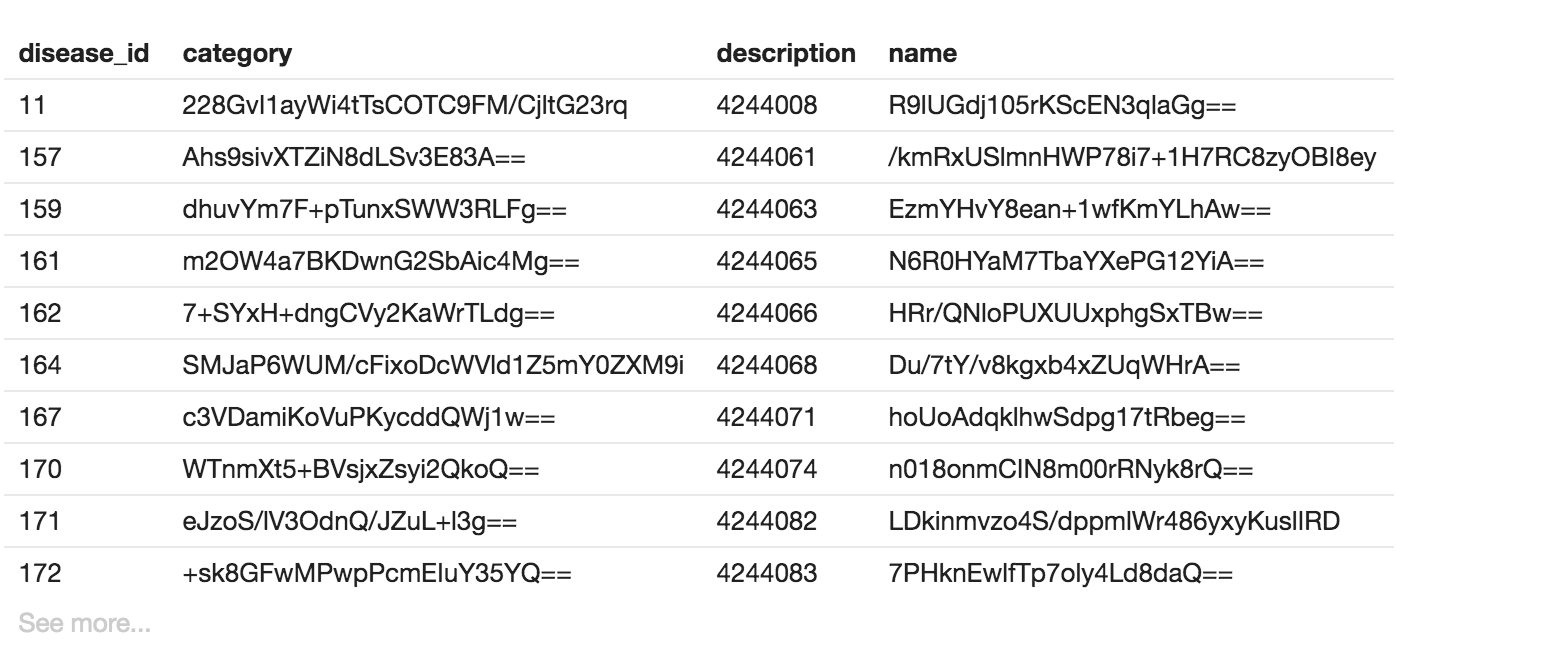
\includegraphics[width=15cm]{pictures/bd-encr}
\caption{Zaszyfrowane krotki bazy danych. Widoczne jest, że ciągi znaków zapisane w bazie danych nie są możliwe do odszyfrowania bez dekodowania.}
\end{figure}

\subsubsection{Ograniczenia}
W trakcie implementacji kolejnych funkcjonalności musieliśmy zmierzyć się z ograniczeniami serwera Heroku. Obsługa zapytań (ang. \textit{request}) jest wykonywana na ograniczonym serwerze, stąd można zaobserwować wydłużony czas oczekiwania na duże zapytanie. Skorzystanie z darmowej domeny sprawia, że funkcjonowanie strony jest po prostu wolne.

\subsubsection{Przyspieszenie}
W trakcie pierwszej wersji implementacji zastosowano wbudowany we framework Spring sterownik będący mostkiem pomiędzy obiektami programu a bazą danych. Jego zastosowanie umożliwiło stosowanie zapytań do bazy przy użyciu specjalnie spreparowanych nazw metod. Wykorzystując ten sposób i np. metodę

\begin{lstlisting}
Optional<Patient> findByUserId(Long userId);
\end{lstlisting}

automatycznie generuje się kod SQL, który odpowiada za znalezienie użytkownika o zadanym ID.

Jest to bardzo wygodne, jednak korzystając z możliwości zbudowania własnego zapytania przy użyciu języka SQL udało się uzyskać \textbf{czterokrotne} przyspieszenie związane ze stosowaniem bardziej złożonych zapytań. Wstrzyknięcie zapytania SQL zaimplementowane jest w następujący sposób:

\begin{lstlisting}
@Query(
value = "select distinct patients.patient_id, 
	my_app_users.* from my_app_users " +
	"join patients\n" +
	"on my_app_users.user_id=patients.user_id",
	nativeQuery = true)
List<PatientInfoTO> findAllPatients();
\end{lstlisting}



\subsubsection{Możliwości dotyczące rozwoju - przyspieszenie}
Przyspieszenie może zostać uzyskane np. poprzez zastosowanie architektury mikro-serwisowej, tak by każda atomowa operacja mogła zostać wykonywana niezależnie. Zapewniłoby to dużą skalowalność systemU i pod dużym obciążeniem przełożyłoby się to na przyspieszenie. 

